La datavisualisation (ou \textit{dataviz}) permet de représenter des données afin d'apporter une aide à la prise de décision. Elle facilite la communication tant en interne qu'en externe d'une entreprise.\\

\begin{figure}[H]
\begin{center}
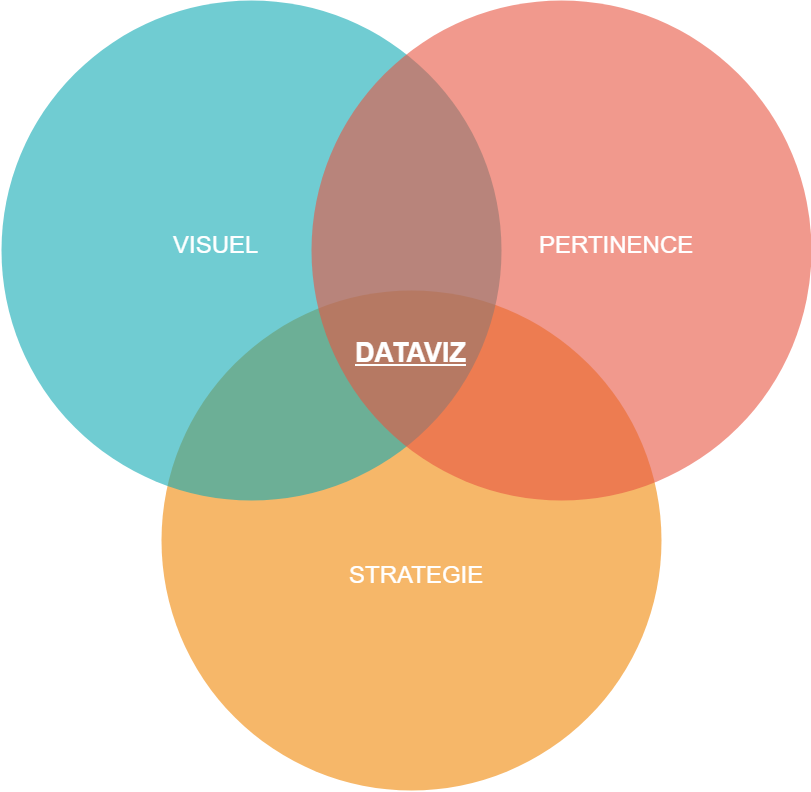
\includegraphics[scale=0.3]{resources/dataviz.png}
\caption{Principes de la datavisualisation}
\end{center}
\end{figure}

C'est un concept qui existe depuis de nombreuses années, bien avant l'arrivée de l'informatique. Elle est cependant très utilisée dans ce domaine au vu du contexte de Big Data qui a émergé ces dernières années.\\

Le phénomène de datavisualisation repose sur des critères visuels, de pertinence de l'information et de la stratégie qui peut en découler, comme présenté dans la figure 4.1. Ces trois critères sont fondamentaux et permettent de qualifier une solution de datavisualisation.\\

Le marché de la datavisualisation est encore en pleine croissance au vu de son émergence récente. Néanmoins, il existe déjà des solutions qui répondent aux besoins des entreprises.